% Copyright 2025 by Lernik Asserian
% This file may be distributed and/or modified.

\documentclass[11pt,letterpaper,reqno]{amsart}
\usepackage{amsmath}
\usepackage{amssymb}
\usepackage{amsthm}
\usepackage{booktabs}
\usepackage{graphicx}
\usepackage{xspace}
\usepackage[dvipsnames]{xcolor}
\usepackage{setspace}
\usepackage[letterpaper,margin=1in,headheight=15pt]{geometry}
\usepackage{bm}
\usepackage{hyperref}
\definecolor{hyperlinkblue}{rgb}{0,0,238}
\hypersetup{colorlinks=true,urlcolor=hyperlinkblue,linkcolor=hyperlinkblue,citecolor=hyperlinkblue}
\allowdisplaybreaks

% Makes the subsection go onto a new line
% \makeatletter
% \def\subsection{\@startsection{subsection}{2}%
%   \z@{.5\linespacing\@plus.7\linespacing}{.5\linespacing}%
%   {\normalfont\bfseries}}
% \makeatother

% Customizing the inclusion of codes in Appendix
\usepackage{listings}
\lstdefinestyle{mystyle}{
    backgroundcolor=\color{lightgray!20}, % A light gray background
    commentstyle=\color{green!60!black},
    keywordstyle=\color{blue},
    numberstyle=\tiny\color{gray},
    stringstyle=\color{purple},
    basicstyle=\fontfamily{pcr}\selectfont\footnotesize, % Use a courier-like font
    breakatwhitespace=false,         
    breaklines=true,                 
    captionpos=b,                    
    keepspaces=true,                 
    numbers=left,                    
    numbersep=5pt,                  
    showspaces=false,                
    showstringspaces=false,
    showtabs=false,                  
    tabsize=2
}
\lstset{style=mystyle}

\numberwithin{equation}{subsection}
\newtheorem{thm}{Theorem}
\newtheorem{lem}[thm]{Lemma}
\newtheorem{prop}[thm]{Proposition}
\newtheorem{cor}[thm]{Corollary}
\theoremstyle{definition}
\newtheorem{Example}[thm]{Example}
\newtheorem{Definition}[thm]{Definition}
\numberwithin{thm}{subsection}
\newtheorem{problem}{Problem}

% labeling of figures and tables
\newcounter{figtab}[subsection]
\setcounter{figtab}{0}
\makeatletter
\@addtoreset{figure}{subsection}
\@addtoreset{table}{subsection}
\makeatother
\renewcommand{\thefigure}{\thesubsection.\arabic{figtab}}
\renewcommand{\thetable}{\thesubsection.\arabic{figtab}}
\let\oldfigure\figure
\def\figure[#1]{\oldfigure[#1]\stepcounter{figtab}}
\let\oldtable\table
\def\table[#1]{\oldtable[#1]\stepcounter{figtab}}

\usepackage{biblatex}
\addbibresource{references.bib}


\begin{document}

\onehalfspacing

\title{How Do Acoustic Features Relate to the Emotions We Hear in Music?}

\author{Caden Che and Kevin Zuniga}

\thanks{
This report is submitted as part of the capstone requirement
for the Mathematics major at Stanford University.
}

\begin{abstract}
This project examines relationships between acoustic measurements and the emotional character of recorded music, represented through valence and arousal. Following an initial electronic-music pilot, we broadened the analysis to music across genres using MERGE. The completed follow-up includes 3,542 recordings and compares seven initial features with an expanded set of 82 measurements describing amplitude, rhythm, timbre, and pitch-class content. Models are evaluated using nested cross-validation grouped by artist credits. Expanded ridge regression obtains held-out $R^2$ values of $0.213$ for valence and $0.415$ for arousal. A random forest gives the strongest performance among the evaluated configurations, reaching $R^2=0.293$ and $R^2=0.494$, respectively. Removing added timbre or pitch-class features increases valence prediction error. These exploratory findings provide a basis for two selected-song case studies comparing perceived sadness and happiness through acoustic measurements and model predictions.
\end{abstract}

\maketitle
\section{Introduction}

Electronic dance music often combines a strong rhythmic pulse with a wide range of emotional character. Our interest in this project developed from listening to songs that we perceive as sad despite their energetic production. This raises a question that can be approached through statistical learning: which musical characteristics help explain the emotional mood of EDM?

We investigate relationships between measured acoustic features and supplied valence and arousal scores. Valence describes emotional positivity, while arousal describes activation. Separating these responses makes it possible to study negative mood alongside energetic sound. It also avoids defining emotional arousal directly from an audio measurement such as loudness or tempo.

The present report analyzes 92 provisional dance-style candidates selected from MERGE Audio Complete. We extract interpretable measurements of amplitude, rhythm, spectral brightness, spectral change, and bass-band content, then fit separate ridge regressions for valence and arousal. Grouped evaluation keeps each complete artist-credit group within a single fold. An exploratory extension measures temporal changes within the excerpts and connects those measurements to the later study of buildups, drops, and breakdowns.

The initial results show a modest improvement over a training-mean baseline for arousal, with the clearest contribution from spectral brightness and spectral change. The same seven-feature model does not improve valence prediction. Coarse temporal descriptors produce small, split-dependent changes in performance. These findings motivate a more targeted examination of musical structure and additional characteristics, especially those related to harmony and melody. The final EDM review and the two personal song case studies remain part of the next phase of the project.

Section 2 reviews the relevant literature. Section 3 defines the model, documents the data selection and implementation, and presents the evaluated results. The conclusion summarizes what these results support and the further evidence needed to address the case-study questions.

\section{Background and Literature Review}
\label{sec:literature}

Music emotion recognition examines how information in a recording relates to its emotional character. Our interest in this topic developed from listening to electronic dance music (EDM), particularly songs that combine a strong rhythmic pulse with a mood we perceive as sad. These examples motivate our research question: which musical characteristics help explain the emotional mood of EDM? We study this question through the relationship between measurable acoustic features and valence and arousal. Previous work informs our choice of emotion labels, data, and methods, as well as the interpretation of the resulting predictions.

\subsection{Defining the emotional response}

Kang and Herremans review music emotion datasets, prediction methods, and evaluation challenges \cite[Secs.~II and V]{kang2025survey}. They distinguish perceived emotion, which describes what a listener hears in a song, from induced emotion, which describes how listening makes that person feel. A listener may enjoy music perceived as sad, illustrating why perceived and induced emotion require different prediction targets. The survey also separates static annotations, which summarize a recording, from dynamic annotations that follow changes over time.

Valence and arousal provide a useful representation for our question. Valence describes emotional positivity, while arousal describes activation, ranging from calm to highly activated. These dimensions let us examine negative mood without assuming that it always appears in slow or quiet music. Tempo, amplitude, and onset activity will be acoustic predictors; the supplied valence and arousal scores will be the responses.

In this study, ``explaining mood'' refers to identifying associations between acoustic measurements and the supplied emotion scores. Low valence can correspond to several negative emotions, including sadness and anger. We therefore interpret the regression response as emotional negativity and use written listening descriptions to discuss sadness more specifically in the case studies.

\subsection{MERGE as a starting point}

Louro et al. introduce MERGE for static emotion prediction using audio, lyrics, and both modalities together \cite[Secs.~III--V]{louro2025merge}. The complete audio release contains 3,554 excerpts, while the bimodal dataset contains 2,216 examples. The authors evaluate four-quadrant classification and numerical valence--arousal regression. Their creation protocol maps AllMusic emotion tags into the valence--arousal plane using affective word ratings and includes manual validation. It also excludes examples close to the center of that plane to reduce ambiguity.

MERGE provides an established framework for feature-based mood prediction. Our study applies that framework to an EDM-focused sample and emphasizes a small set of interpretable acoustic measurements. We will examine which features are associated with valence, which are associated with arousal, and how well those relationships predict held-out examples. The contribution of our study is the interpretation of these relationships within a defined EDM sample and their application to selected case-study recordings.

The annotation procedure determines the meaning of the response variables. Our models will predict scores derived through MERGE's construction process; the study does not collect a new set of listener ratings. In addition, genre metadata must be reviewed before defining our final population. An Electronic tag is useful for screening, but it covers a broader category than the dance-music population of interest. Section~\ref{sec:selection} gives the reproduced counts and selection rules.

\subsection{EDM production and emotional intensity}

Solberg examines production techniques in buildup and drop sections through descriptive and interpretive musical analysis \cite{solberg2014bass}. The discussion connects techniques such as drum rolls, frequency changes, contrasting breakdowns, and the removal and return of bass to expectation, tension, and emotional intensity. This work gives a musical basis for examining rhythmic activity, low-frequency content, and changes in amplitude and timbre.

For our analysis, this work motivates a distinction between emotional intensity and emotional positivity. A production change that builds anticipation could be relevant to arousal without having the same relationship with valence. We will investigate that possibility by fitting separate models for the two responses. The temporal resolution of the data also limits the analysis. Features averaged over a short excerpt summarize the audio in that interval and do not describe a complete buildup-to-drop sequence. Our initial models will therefore relate excerpt-level measurements to supplied static labels.

\subsection{What separate musical sources can tell us}

In EmoMucs, de Berardinis, Cangelosi, and Coutinho use source separation to estimate vocals, bass, drums, and other accompaniment, then compare source-specific prediction models and fusion strategies \cite[Secs.~3--4]{deberardinis2020emomucs}. Their experiments use PMEmo's static induced-emotion annotations. In one configuration, valence $R^2$ improves from $0.4143$ for the full-mix baseline to $0.4814$ when source predictions are combined. Arousal performance is comparable to the baseline. Individual source models perform less well than the full mix, and the best source varies across tracks.

These findings suggest that mood-related information can be distributed across musical components and that source usefulness depends on the recording. The use of induced-emotion annotations also distinguishes EmoMucs from MERGE's perceived-mood framework. Its reported scores provide methodological context, rather than a directly comparable performance benchmark for our sample.

Our initial models use measurements defined on the complete audio mix. For example, low-frequency power can contain contributions from bass instruments, kick drums, and other sounds. We describe this quantity as bass-band content. A comparison of separated sources would constitute a subsequent experiment requiring assessment of separation quality.

\subsection{Source separation and learned representations}

Hybrid Transformer Demucs estimates musical sources using waveform and spectrogram information, with a transformer connecting the representations \cite{rouard2023demucs}. Its task is source reconstruction, and its separation scores measure reconstruction quality. This method could support a subsequent comparison of acoustic features across estimated stems. Those estimates may contain leakage or distortion, particularly where kick drums and synthesizer bass overlap. Representative outputs would require listening-based quality checks before an estimated stem could be interpreted as an instrument-specific measurement.

MERT offers a complementary approach based on learned audio representations. Li et al. learn numerical music representations through self-supervised training with acoustic and pitch-related targets, then evaluate the representations on downstream music tasks \cite{li2024mert}. A frozen representation could be paired with a small prediction model when labeled data are limited. Its coordinates, however, do not have the direct meanings of quantities such as tempo or spectral centroid. Explicit acoustic features provide a more direct connection between a fitted prediction and a named musical characteristic, which is central to our research question. Demucs and MERT are therefore relevant methodological options rather than parts of the completed preliminary analysis.

\subsection{Other data and the resulting study design}

DEAM provides 1,802 excerpts and full songs with valence and arousal annotations both over time and at the recording level \cite{deamdataset}. It is a possible source of additional examples if our final EDM subset is small. Before combining it with MERGE, we would need to check genre coverage, identify repeated recordings, align label scales, and examine differences in annotation procedures. Matching numerical ranges alone would not establish that the labels measure the same target. We have not pooled these datasets in the present audit.

Taken together, these studies support a feature-based regression design with separate valence and arousal responses. We will use grouped evaluation to test whether the learned relationships extend to held-out recordings and compare performance with a training-mean baseline. The fitted models will then be applied to excerpts from two EDM songs selected as case studies. For each excerpt, we will examine the features contributing to its predicted valence and arousal and compare the prediction with a written listening description. These examples will illustrate both the interpretability of the fitted relationships and information that may be absent from the initial feature set, including harmony, lyrical meaning, and structural context.

\section{Methodology and Technical Implementation}
\label{sec:methodology}
\subsection{Mathematical Model}
\label{sec:model}

We specify two ridge regression models for the relationship between acoustic characteristics and emotional mood. For excerpt $i$, let $v_i$ and $a_i$ denote its supplied valence and arousal scores. We model these responses separately because a recording can combine low valence with high arousal. Separate response models allow the same acoustic characteristic to have different associations with emotional positivity and activation.

\subsubsection{Predictors and responses}
Let $n$ denote the number of eligible excerpts in the finalized sample, and let $\bm{x}_i\in\mathbb{R}^7$ contain the measurements listed in Table~\ref{tab:predictors}. These seven features were extracted in the preliminary analysis; final inclusion depends on the genre review and feature checks. No mood tags, quadrant labels, or other emotion-derived metadata will be used as predictors. The released numerical labels we inspected lie on a $[0,1]$ scale. We will preserve that scale and document it alongside the annotation procedure.

\begin{table}[ht]
\centering
\caption{Initial acoustic predictors, computed from each excerpt.}
\label{tab:predictors}
\begin{tabular}{ll}
\toprule
Measurement & Musical interpretation \\
\midrule
Mean frame RMS amplitude & Typical signal amplitude \\
Standard deviation of frame RMS & Variation in signal amplitude \\
Mean spectral centroid (Hz) & Spectral brightness \\
Power fraction in $20\leq f<250$ Hz & Bass-band content \\
Mean positive spectral flux & Changes in spectral magnitude \\
Detected onsets per second & Rate of detected sound attacks \\
Estimated tempo (BPM) & Estimated beat rate \\
\bottomrule
\end{tabular}
\end{table}

RMS amplitude describes signal amplitude and serves as an approximate loudness-related measurement. Estimated tempo is subject to beat-tracking errors. Bass-band content measures the proportion of spectrogram power in the stated frequency range. These quantities describe aspects of the audio; arousal remains a response label. Harmony and mode are possible later additions, but we have not yet validated features that would support claims about minor chords.

\subsubsection{Defining the audio measurements}

The preliminary extraction converts audio to mono at $22{,}050$ samples per second. It uses a short-time Fourier transform with a Hann window of length $N=2{,}048$ and a hop length of $512$ samples. Let $S_{kt}\geq0$ denote the resulting magnitude at frequency bin $k$ and frame $t$, with frequency $f_k$. Let $L$ be the number of frames and $T$ the excerpt duration in seconds.

For the windowed samples $u_{t\ell}$ in a frame, its RMS amplitude is
\begin{equation}
 R_t=\sqrt{\frac{1}{N}\sum_{\ell=0}^{N-1}u_{t\ell}^2}.
\end{equation}
The extraction computes the equivalent quantity from the spectrogram. Its two summaries are
\begin{equation}
 \overline R=\frac{1}{L}\sum_{t=1}^{L}R_t,
 \qquad
 s_R=\sqrt{\frac{1}{L}\sum_{t=1}^{L}(R_t-\overline R)^2}.
\end{equation}
Here $s_R$ is a population standard deviation across frames. Both measurements depend on the recording's amplitude scale and production, which matters when comparing mastered tracks.

The spectral centroid for a non-silent frame is
\begin{equation}
 C_t=\frac{\sum_k f_k S_{kt}}{\sum_k S_{kt}},
 \qquad \overline C=\frac{1}{L}\sum_{t=1}^{L}C_t.
\end{equation}
Silent frames are assigned centroid zero in the extraction. Larger values indicate that spectral magnitude is concentrated at higher frequencies. The bass-band fraction is
\begin{equation}
 B=\frac{\sum_t\sum_{k:\,20\leq f_k<250}S_{kt}^2}
 {\sum_t\sum_k S_{kt}^2}.
\end{equation}
The implementation adds a small constant to the denominator to handle near-silence. Positive spectral flux is summarized by
\begin{equation}
 F=\frac{1}{L-1}\sum_{t=2}^{L}\sum_k
 \max\{S_{kt}-S_{k,t-1},0\}.
\end{equation}
This particular flux measure uses unnormalized spectral magnitudes, so amplitude changes can affect it. We will inspect its correlation with the RMS features before interpreting its coefficient.

If the onset detector identifies $D$ attacks, the onset-rate feature is $D/T$. The tempo estimate is the beat-rate estimate returned by the audio analysis algorithm, measured in BPM. Onset rate and tempo describe different aspects of rhythm: a recording can contain several detected attacks within one beat. We will inspect beat-tracking errors, including estimates at half or twice a plausible tempo. All case-study excerpts will use this same feature-extraction procedure.

For training-set size $m$, define the standardized predictor
\begin{equation}
 z_{ij}=\frac{x_{ij}-\mu_j}{s_j},
 \qquad j=1,\ldots,p,
\end{equation}
where $\mu_j=m^{-1}\sum_{i=1}^m x_{ij}$ and $s_j=\{m^{-1}\sum_{i=1}^m(x_{ij}-\mu_j)^2\}^{1/2}$ are the training mean and standard deviation. Constant predictors are removed, so $p\leq7$. The same training values are used to transform held-out songs. A coefficient $\beta_{jr}$ therefore represents the fitted change in response $r$ associated with a one-training-standard-deviation increase in predictor $j$, holding the other standardized predictors fixed.

\subsubsection{Ridge estimation}

Ridge regression adds a squared-coefficient penalty to least squares; van Wieringen reviews this framework and its properties \cite{vanwieringen2026ridge}. Below we derive the estimator using our chosen normalization of the loss.
For response index $r\in\{v,a\}$, define $y_{iv}=v_i$ and $y_{ia}=a_i$. The model is
\begin{equation}
 y_{ir}=\beta_{0r}+\bm{z}_i^{\mathsf T}\bm{\beta}_r+\varepsilon_{ir}.
 \label{eq:linear}
\end{equation}
We estimate the coefficients by minimizing
\begin{equation}
 (\widehat\beta_{0r},\widehat{\bm\beta}_r)
 =\operatorname*{arg\,min}_{b,\bm\beta}
 \left\{\frac{1}{m}\sum_{i=1}^{m}
 (y_{ir}-b-\bm z_i^{\mathsf T}\bm\beta)^2
 +\lambda_r\lVert\bm\beta\rVert_2^2\right\},\qquad\lambda_r>0.
 \label{eq:ridge}
\end{equation}
The intercept is unpenalized. The penalty limits coefficient size, which is useful because measurements such as amplitude and onset activity may be correlated. Equation~\eqref{eq:linear} is a linear approximation to the relationship between the chosen measurements and the supplied labels. The residual term includes both variation not captured by these predictors and error in the measurements or labels.

\begin{prop}
For any $\lambda_r>0$, problem~\eqref{eq:ridge} has a unique solution, even if the standardized predictors are linearly dependent.
\end{prop}
\begin{proof}
Let $Z$ be the $m\times p$ training matrix with centered columns and let $\bm y_{c,r}=\bm y_r-\bar y_r\bm 1$. The derivative with respect to the intercept is $-2m^{-1}\sum_i(y_{ir}-b-\bm z_i^{\mathsf T}\bm\beta)$. Since $\sum_i\bm z_i=\bm0$, setting it to zero gives $\widehat\beta_{0r}=\bar y_r$. The normal equations for the remaining coefficients are
\[
 (Z^{\mathsf T}Z+m\lambda_r I_p)\widehat{\bm\beta}_r
 =Z^{\mathsf T}\bm y_{c,r}.
\]
For every nonzero $\bm u\in\mathbb R^p$,
\[
 \bm u^{\mathsf T}(Z^{\mathsf T}Z+m\lambda_r I_p)\bm u
 =\lVert Z\bm u\rVert_2^2+m\lambda_r\lVert\bm u\rVert_2^2>0.
\]
The matrix is positive definite and invertible. Thus
\[
 \widehat{\bm\beta}_r
 =(Z^{\mathsf T}Z+m\lambda_r I_p)^{-1}Z^{\mathsf T}\bm y_{c,r},
\]
and both the coefficient vector and intercept are unique.
\end{proof}

\begin{prop}
Let $q=\operatorname{rank}(Z)$ and let $Z=UDV^{\mathsf T}$ be a compact singular value decomposition, where $U\in\mathbb R^{m\times q}$ and $V\in\mathbb R^{p\times q}$ have orthonormal columns and $D=\operatorname{diag}(d_1,\ldots,d_q)$ has positive entries. Then the fitted centered training response satisfies
\begin{equation}
 Z\widehat{\bm\beta}_r
 =U\,\operatorname{diag}\!\left(
 \frac{d_\ell^2}{d_\ell^2+m\lambda_r}
 \right)_{\ell=1}^{q}U^{\mathsf T}\bm y_{c,r}.
\end{equation}
Each represented direction is shrunk by a factor strictly between zero and one. The factors approach zero as $\lambda_r$ tends to infinity.
\end{prop}
\begin{proof}
Substitute $Z=UDV^{\mathsf T}$ into the ridge solution. On the column space of $V$, the matrix $Z^{\mathsf T}Z+m\lambda_r I_p$ acts as $D^2+m\lambda_r I_q$. Multiplying the solution on the left by $Z$ therefore gives
\[
 Z\widehat{\bm\beta}_r
 =UD(D^2+m\lambda_r I_q)^{-1}DU^{\mathsf T}\bm y_{c,r}.
\]
The diagonal entries are $d_\ell^2/(d_\ell^2+m\lambda_r)$. Positivity of $d_\ell$ and $\lambda_r$ proves the stated bounds and limit. If $Z$ has rank zero, the centered fitted response is zero.
\end{proof}

The shrinkage formula gives a direct interpretation of the regularization penalty. Directions with small singular values receive stronger shrinkage at the same penalty value. Increasing the penalty eventually brings predictions toward the training-mean intercept. We will choose the penalty through validation because the best balance between flexibility and stability depends on the data.

\subsubsection{Evaluation and interpretation}
We will use grouped cross-validation, keeping excerpts and repeated versions of the same recording together. Artist-held-out evaluation will help assess whether patterns extend beyond artists represented in training. Within each outer training fold, an inner grouped validation procedure will choose $\lambda_r$ from the grid $\{10^{-4},10^{-3},\ldots,10^4\}$. Feature scaling and any imputation will be fitted inside the corresponding training fold. The number of folds will be chosen after checking the number of eligible groups. No case-study excerpts will be used to tune the models.

For held-out predictions, we will report
\begin{equation}
 \mathrm{RMSE}_r=
 \sqrt{\frac{1}{n_{\mathrm{test}}}\sum_{i\in\mathrm{test}}
 (y_{ir}-\widehat y_{ir})^2}.
\end{equation}
We will compare this error with a baseline that predicts the outer training mean. Ridge predictions can fall outside $[0,1]$; we will report their frequency and evaluate the raw predictions consistently. Coefficients will be summarized across outer folds to show whether their signs and magnitudes are stable. To assess predictive usefulness, we will also refit and retune models with each feature family omitted, using the same outer folds. Correlated predictors can substitute for one another, so a small error change does not establish that a musical characteristic is irrelevant.

We will group the predictors into amplitude ($\overline R,s_R$), rhythm (onset rate and tempo), spectral change and brightness ($F,\overline C$), and bass-band content ($B$). For family $g$, define the held-out error change
\begin{equation}
 \Delta_{g,r}=\mathrm{RMSE}_{r,-g}-\mathrm{RMSE}_{r,\mathrm{full}}.
\end{equation}
A positive value indicates that omitting the family worsens prediction under the stated evaluation procedure. We will report the changes across folds as well as the aggregate value. A negative value is possible if the omitted features add noise or do not generalize. These comparisons will complement coefficient summaries rather than provide a ranking of causal effects.

We will also report out-of-fold $R^2$:
\begin{equation}
 R^2_r=1-\frac{\sum_i(y_{ir}-\widehat y^{\mathrm{OOF}}_{ir})^2}
 {\sum_i(y_{ir}-\bar y_r)^2},
\end{equation}
provided the response has nonzero variation. Here each prediction is obtained from an outer model that did not train on that example, and $\bar y_r$ is the mean of the evaluated responses. This statistic can be negative and is not a classification accuracy. The training-mean baseline will still be evaluated separately in every outer fold, since it is the deployable constant predictor for that fold.

\subsubsection{Case-study predictions}
After evaluation, the model will be refitted on the eligible study sample using grouped validation to select its penalty. The case-study recordings will remain excluded from all training and tuning. For a case-study excerpt $\ast$, define $c_{jr}=\widehat\beta_{jr}z_{\ast j}$. Then
\begin{equation}
 \widehat y_{\ast r}-\widehat\beta_{0r}
 =\sum_{j=1}^{p}c_{jr}.
 \label{eq:contributions}
\end{equation}
This identity gives an exact decomposition of the fitted linear prediction relative to its training-mean intercept. A negative valence contribution indicates that a measured feature lowers the model's prediction for that excerpt. The contribution describes an association within the fitted model. Establishing a causal effect of changing the musical characteristic would require an experimental design beyond the scope of this study. Each case study will use a prespecified excerpt of approximately 30 seconds, identified by its timestamp before model predictions are inspected. We will check whether its standardized features lie within the observed training ranges and compare the predicted valence and arousal with an independently written listening description. We will report the intercept, individual feature contributions, and residual difference if a comparable emotion annotation is available. An informal description alone will not be treated as a numerical ground-truth score. Prediction errors will remain part of the case-study analysis and will be discussed in relation to the coverage of the feature set and the training sample.

\subsection{Data Collection and Analysis}
\label{sec:selection}

MERGE Audio Complete, version 1.1.0, is the primary data source for this project \cite{mergedata}. The release contains audio excerpts, descriptive metadata, and supplied emotion labels. Its complete audio collection provides a broader starting point than the bimodal subset, since the present analysis does not require lyrics.

Our initial review examined electronic and dance-related metadata to identify a sample appropriate to the original EDM question. The revised question considers recordings across genres. The final selection procedure will document usable audio, available response labels, repeated recordings, and the relationship between recording identifiers and artist credits.

We also considered DEAM because it provides both recording-level and time-varying valence and arousal annotations \cite{deamdataset}. Its temporal labels could support a later analysis of emotional changes within recordings. DEAM has not been pooled with MERGE in the completed analysis.

\subsection{Implementation}
\label{sec:implementation}

\subsubsection{Audio preparation and eligibility}

The follow-up uses the official MERGE Audio Complete archive. Its MD5 checksum was verified before extraction. Metadata and numerical response tables were joined one-to-one using the \texttt{Song} identifier.

The release contains 3,554 identifiers. For the completed evaluation, we excluded four records without artist credits, six additional records repeating normalized artist/title pairs, one further exact audio-file duplicate, and one excerpt that failed the minimum six-second extraction requirement. These rules leave 3,542 recordings and 1,755 normalized complete artist-credit groups.

Repeated artist/title pairs were handled conservatively by retaining the first identifier after sorting by \texttt{Song}. Exact audio duplicates were identified using file hashes. The eligibility decisions were recorded before evaluating the broader models.

\subsubsection{Acoustic feature extraction}

Audio was converted to mono at 22,050 samples per second. Spectral measurements used a short-time Fourier transform with a 2,048-sample window and a 512-sample hop.

The initial seven features were retained for comparison. The expanded representation added the measurements in Table~\ref{tab:features}, producing 82 acoustic predictors. The pitch-class summaries describe chroma entropy, changes in chroma, and the triad-template contrast in Equation~\eqref{eq:triad}.

For the LSTM, each excerpt was divided into ten equal-duration windows. Four acoustic measurements were calculated in each window, producing a sequence with ten time steps. These windows share the recording's overall response pair and are not treated as independently labeled examples.

Artist, title, genre, mood tags, quadrant labels, and other emotion-derived metadata were excluded from the predictor matrices. Artist credits were used only to define evaluation groups. All retained acoustic measurements and response values were checked for missing or non-finite values.

\subsubsection{Training and parameter selection}

The primary evaluation used random seed 195. Each outer training partition was divided into three grouped inner folds. Standardization and model tuning used only the relevant training data.

For each candidate parameter setting, inner validation errors were pooled across the three folds. The setting with the lowest pooled mean squared error was refitted on the outer training partition and used to predict the held-out outer fold.

Random-forest tuning compared minimum leaf sizes of three and eight and feature fractions of $0.5$ and $1.0$. The RBF approximation compared penalties of $0.01$, $0.1$, $1$, and $10$ and kernel widths of $0.001$, $0.01$, and $0.1$. The LSTM used the fixed settings described in Section~\ref{sec:model}.

We also evaluated a static-model selection procedure. Within each outer training partition, it selected among the candidate static model families using their inner validation scores. The outer test results were reserved for evaluation.

\subsubsection{Checks and external-song refits}

Checks confirmed that no normalized artist-credit group crossed an outer training/test boundary. Every evaluated model produced a held-out prediction for each retained recording and response. Expanded ridge was additionally evaluated using seeds 196 and 197 to examine sensitivity to group assignment.

After evaluation, expanded ridge and random-forest models were refitted for later external-song predictions. Their training predictions were not used as estimates of predictive performance.

The case-study procedure applies the same feature definitions to a selected excerpt, uses the saved training-based scaling, and reports predicted valence and arousal. Ridge contributions are calculated using Equation~\eqref{eq:contributions}. These terms explain the ridge output only and are not a decomposition of the random-forest prediction.

The procedure also checks for known training identifiers, exact training-audio matches, and measurements outside the observed training ranges. Actual predictions for the two selected case-study songs remain pending.

\subsection{Results}
\label{sec:results}

\subsubsection{Prediction of valence and arousal}

The primary seven-feature model produced a modest improvement for arousal and no improvement for valence in the provisional sample. Table~\ref{tab:performance} reports pooled out-of-fold errors, so every evaluated prediction comes from a model that excluded the corresponding artist-credit group. The predictions are evaluated on the supplied numerical label scale. No primary ridge predictions fell outside $[0,1]$.

\begin{table}[ht]
\centering
\caption{Primary grouped evaluation on 92 provisional dance-style excerpts. Lower RMSE and MAE indicate smaller errors. The responses are evaluated separately.}
\label{tab:performance}
\begin{tabular}{llrrr}
\toprule
Response & Method & RMSE & MAE & $R^2$ \\
\midrule
Valence & Training mean & 0.1828 & 0.1612 & -0.007 \\
Valence & Ordinary least squares & 0.1935 & 0.1637 & -0.128 \\
Valence & Ridge & 0.1873 & 0.1651 & -0.057 \\
Arousal & Training mean & 0.0992 & 0.0726 & -0.001 \\
Arousal & Ordinary least squares & 0.0945 & 0.0690 & 0.090 \\
Arousal & Ridge & 0.0931 & 0.0682 & 0.118 \\
\bottomrule
\end{tabular}
\end{table}

For arousal, ridge reduced RMSE from 0.0992 for the training-mean baseline to 0.0931, a relative reduction of approximately 6.2\%. Its out-of-fold $R^2$ was 0.118. For valence, ridge RMSE was 0.1873, compared with 0.1828 for the baseline, and $R^2$ was -0.057. Thus the measured acoustic summaries provided some useful information about activation under this evaluation, but they did not improve the prediction of emotional positivity.

\begin{figure}[ht]
\centering
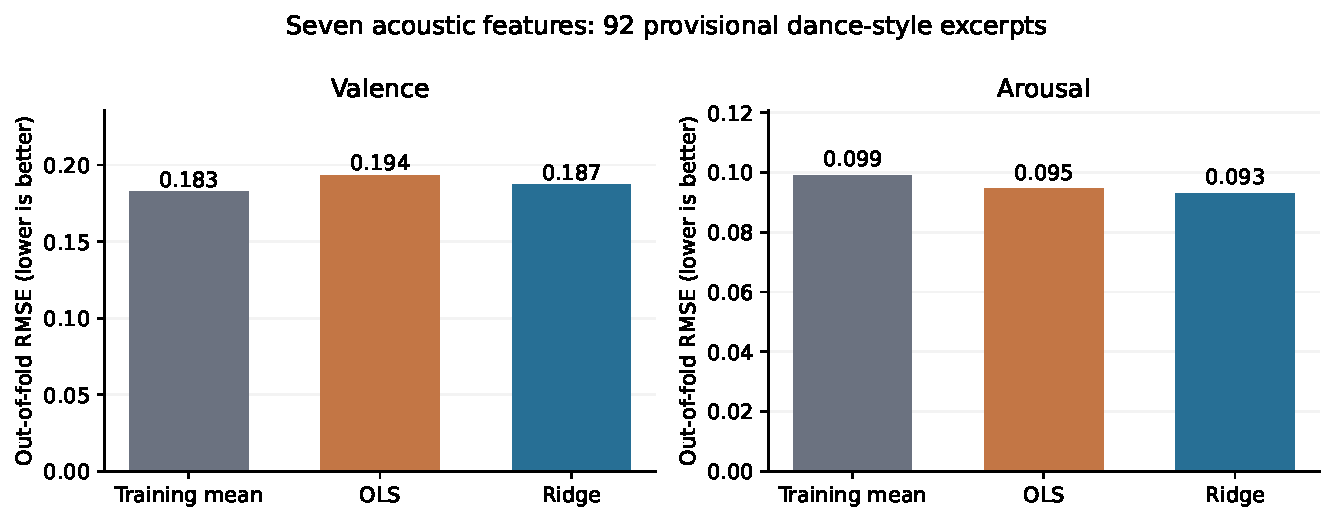
\includegraphics[width=\linewidth]{figures/01_prediction_error.pdf}
\caption{Out-of-fold prediction errors for the training-mean baseline, ordinary least squares, and ridge regression. Each panel begins at zero; the panels have different vertical scales.}
\label{fig:error}
\end{figure}

The numerical error magnitudes should not be compared directly across responses because the supplied arousal scores vary less than the valence scores. Baseline comparisons and $R^2$ are more informative for this purpose. Ordinary least squares also improved on the arousal baseline but had larger error than ridge. Both regression approaches performed worse than the baseline for valence.

\begin{figure}[ht]
\centering
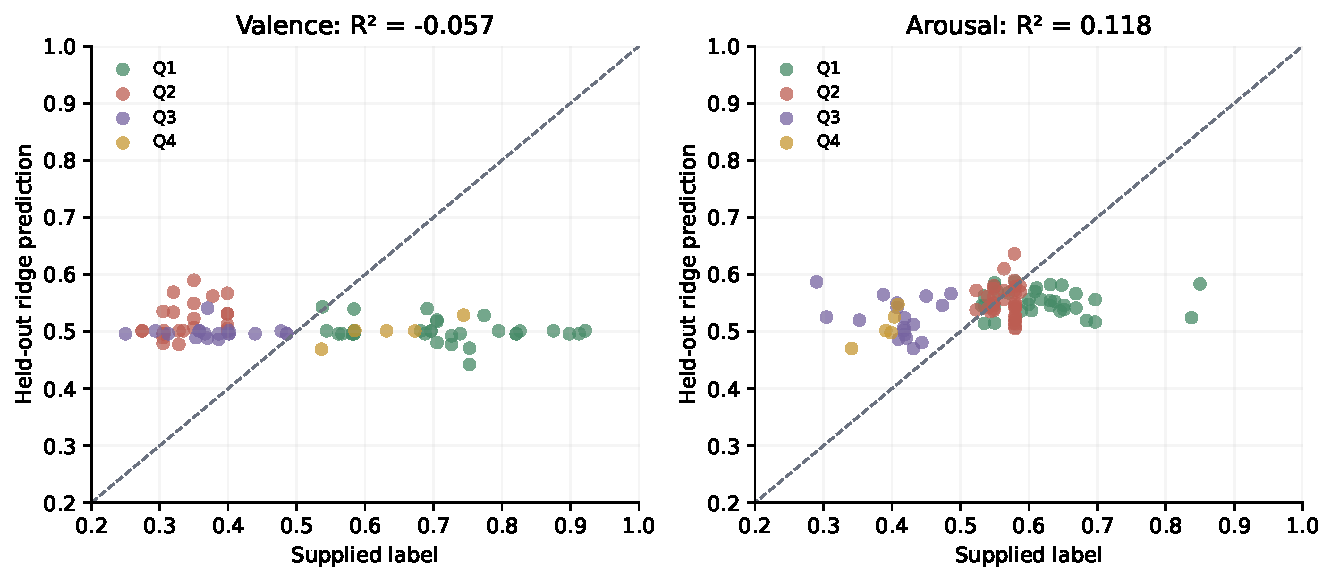
\includegraphics[width=\linewidth]{figures/02_observed_predicted.pdf}
\caption{Supplied labels versus held-out ridge predictions. The dashed line represents perfect prediction. Colors identify the supplied mood quadrants. Points illustrate the restricted range of many predictions, especially for valence.}
\label{fig:predictions}
\end{figure}

The valence predictions are concentrated near the middle of the observed label range. Inner validation selected the largest penalty, $\lambda=10^4$, in three of the five outer folds, leaving these fits close to their training means. This supports a limited interpretation: the seven predictors did not provide sufficiently useful valence information to justify a more flexible linear fit in those folds. It does not imply that valence cannot be predicted from music, since harmony, melodic characteristics, lyrics, and richer representations are absent from this model.

\subsubsection{Which measurements provide useful information?}

Spectral brightness and positive spectral flux had positive arousal coefficients in all five outer models. Their coefficient ranges are shown in Figure~\ref{fig:coefficients}. These are fitted associations conditional on the other measurements. Since predictors are correlated and the penalty changes across folds, coefficient magnitude alone is not a complete measure of predictive usefulness.

\begin{figure}[ht]
\centering
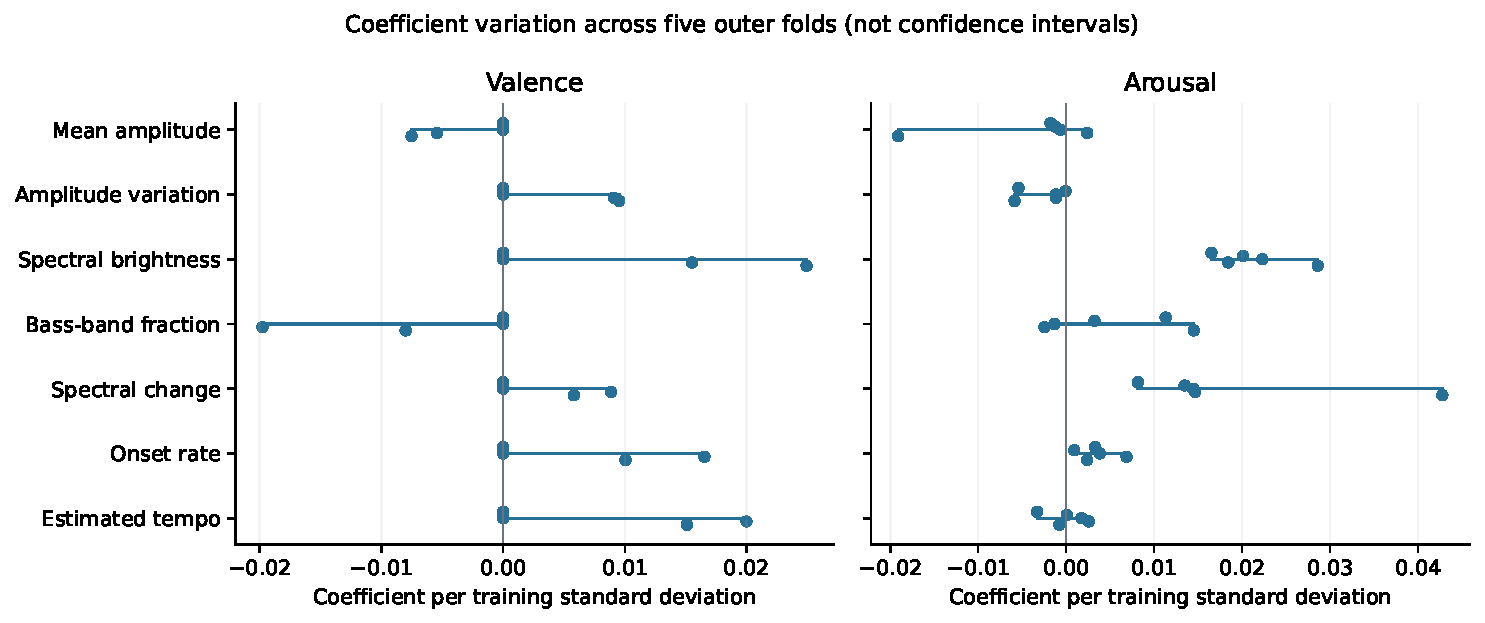
\includegraphics[width=\linewidth]{figures/03_fold_coefficients.pdf}
\caption{Standardized coefficients from the five outer ridge fits. Each dot is a fold-specific estimate, and the line shows the observed range. These ranges describe split variation and are not confidence intervals.}
\label{fig:coefficients}
\end{figure}

We therefore also removed each feature family and refitted and retuned the remaining model. Table~\ref{tab:ablation} reports the aggregate held-out error changes. Omitting brightness and spectral change increased arousal RMSE by approximately $0.0074$, from about $0.0931$ to $0.1004$. It worsened arousal prediction in each outer fold. This was the clearest family-removal effect in the primary analysis. Omitting bass-band content produced a smaller aggregate increase of about $0.0014$, with mixed fold-level effects. Omitting amplitude or rhythm slightly lowered aggregate arousal error in this split. For valence, all aggregate changes were small and the full model itself did not outperform the baseline.

\begin{table}[ht]
\centering
\caption{Change in pooled out-of-fold RMSE after omitting a feature family and retuning. Positive values mean worse prediction than the full ridge model.}
\label{tab:ablation}
\begin{tabular}{lrr}
\toprule
Omitted family & Valence change & Arousal change \\
\midrule
Amplitude & +0.0003 & -0.0005 \\
Rhythm & -0.0013 & -0.0010 \\
Brightness/change & -0.0012 & +0.0074 \\
Bass band & +0.0007 & +0.0014 \\
\bottomrule
\end{tabular}
\end{table}

\begin{figure}[ht]
\centering
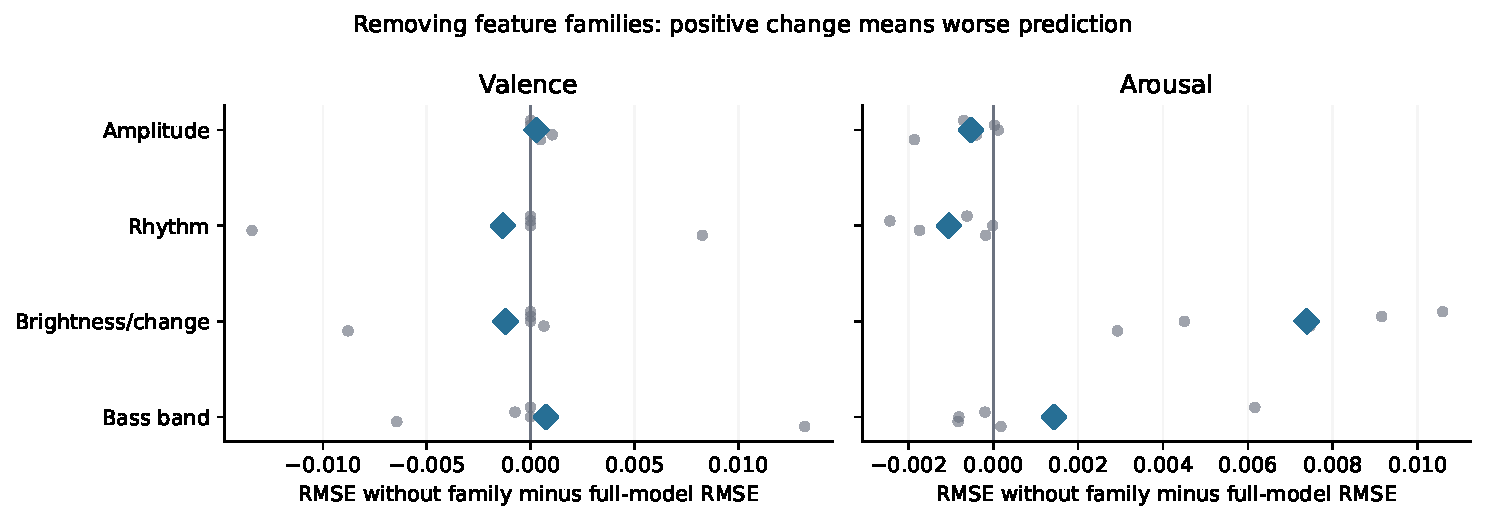
\includegraphics[width=\linewidth]{figures/04_feature_family_ablation.pdf}
\caption{Feature-family removal results. Diamonds show changes in aggregate RMSE; smaller dots show changes within individual outer folds. The fold results do not form independent samples.}
\label{fig:ablation}
\end{figure}

The descriptive correlations provide a compatible, less controlled view. Spectral centroid correlated with arousal at approximately $0.481$, and positive spectral flux at approximately $0.371$. Estimated tempo had an arousal correlation close to zero, approximately $-0.003$. These are excerpt-level correlations in the selected sample, without adjustment for genre composition or artist identity. They should not be interpreted as evidence that changing tempo has no effect on emotion. Beat-tracking errors, production choices, and the limited sample can all affect this relationship.

\subsubsection{Sensitivity to artist-credit group splits}

Across ten grouped split seeds, ridge improved arousal RMSE relative to the corresponding training-mean baseline in all ten evaluations. Arousal $R^2$ ranged from -0.066 to 0.176. Valence ridge RMSE was worse than its baseline in nine of the ten evaluations, and its $R^2$ ranged from -0.115 to -0.013. The overall direction is therefore more stable than the exact score, particularly for arousal. These ranges describe sensitivity to overlapping partitions of the same 92 observations and are not independent-sample confidence intervals.

An additional summary weights each artist-credit group equally by averaging squared errors within a group and then across groups. In the primary split, equal-group arousal RMSE was approximately $0.1011$ for ridge and $0.1074$ for the baseline. Equal-group valence RMSE was approximately $0.1941$ for ridge and $0.1903$ for the baseline. This check preserved the direction of the main comparison while reducing the influence of artists with several excerpts.

\subsubsection{Temporal variation and EDM structure}

The additional temporal analysis examines a musically important question: whether the way the sound changes within an excerpt adds information beyond its average characteristics. The twelve-feature model adds the three time slopes and two adjacent-bin changes defined in Section~\ref{sec:model}. It retains the same static responses and the same outer grouping.

In the primary split, the temporal model obtained valence RMSE 0.1863 and $R^2=-0.045$, and arousal RMSE 0.0926 and $R^2=0.126$. These errors are slightly smaller than those of the seven-feature model. Across ten split seeds, however, the temporal extension improved on the seven-feature model in 3 evaluations for valence and 8 for arousal. The direction varied between partitions. We therefore found no consistent evidence that this particular set of coarse temporal descriptors adds substantial predictive value. This extension was introduced after examining the primary analysis and should be treated as exploratory.

\begin{figure}[ht]
\centering
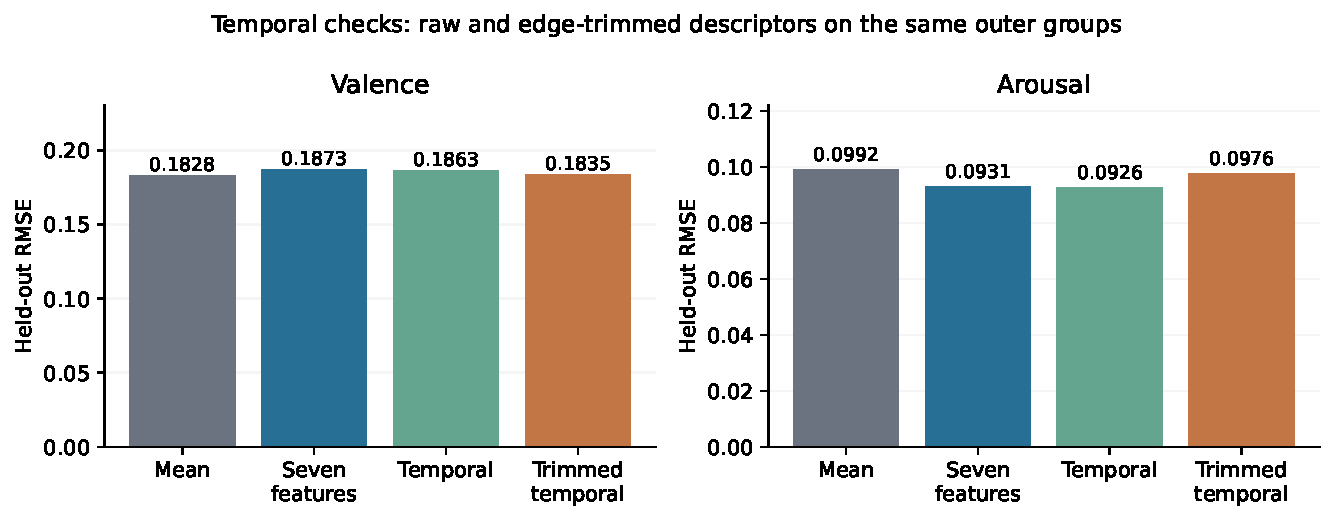
\includegraphics[width=\linewidth]{figures/08_temporal_model_comparison.pdf}
\caption{Primary-split errors for the baseline, seven-feature model, raw temporal extension, and edge-trimmed temporal diagnostic. The temporal checks are exploratory; small improvements were not consistently reproduced across group assignments.}
\label{fig:temporalcomparison}
\end{figure}

Figure~\ref{fig:profiles} shows two examples selected by the largest adjacent-bin increase in amplitude, independently of prediction accuracy. The excerpt from The Prodigy's \emph{We Are the Ruffest} had a maximum increase of approximately $24.34$ dB between adjacent bins, while Fennesz's \emph{Transit} had an increase of approximately $17.33$ dB. These values compare averaged amplitudes in adjacent bins of roughly three seconds. They can be affected by pauses, fades, editing, and other acoustic changes. They are not validated measurements of a drop's intensity.

\begin{figure}[ht]
\centering
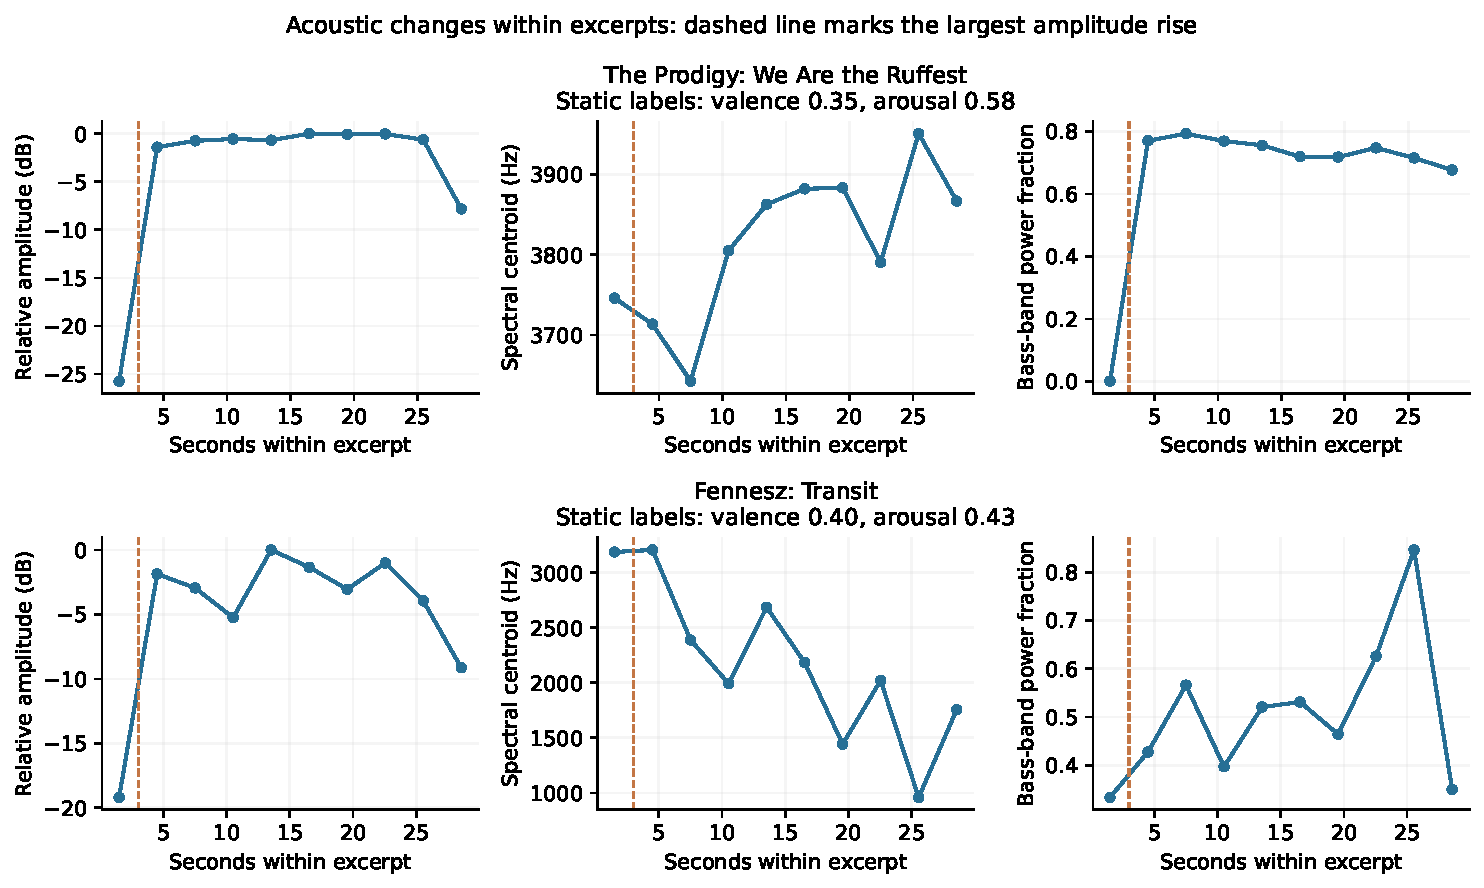
\includegraphics[width=\linewidth]{figures/07_temporal_profiles.pdf}
\caption{Ten-bin acoustic profiles for two descriptively selected examples. The dashed line marks the boundary with the largest increase in bin-average amplitude. Its position does not constitute a confirmed buildup or drop boundary. Each recording has one supplied static emotion pair, not separate emotion labels for the plotted bins.}
\label{fig:profiles}
\end{figure}

To connect these measurements to musical structure, Table~\ref{tab:sections} gives operational cues for later manual annotation. These cues guide listening and feature comparisons; they are not outputs of a trained section detector. A meaningful buildup-to-drop analysis requires the preceding context and a confirmed transition. A 30-second excerpt may contain only part of a section or begin after the transition has occurred.

\begin{table}[ht]
\centering
\caption{Proposed listening cues and measurements for annotated case-study sections. These are analysis criteria, not section labels assigned to the 92 excerpts.}
\label{tab:sections}
\begin{tabular}{p{0.15\linewidth}p{0.35\linewidth}p{0.38\linewidth}}
\toprule
Section & Listening cue to review & Measurement to compare \\
\midrule
Breakdown & Reduced rhythmic activity relative to neighboring sections & Onset rate, amplitude, and bass-band content \\
Buildup & Accumulation of rhythmic or spectral activity before a transition & Time slopes of onset rate and brightness \\
Drop & Re-entry or change in the main rhythmic and low-frequency texture & Changes relative to the preceding buildup \\
Core & A comparatively sustained groove or texture & Feature levels and within-section variation \\
\bottomrule
\end{tabular}
\end{table}

The case-study code can calculate features from independently annotated sections and express the difference between their model-input predictions as a sum of feature changes. A valid listening claim about emotional change would additionally require section-level emotion annotations. Consequently, the present results concern acoustic variation associated with an overall mood score. We have not established how perceived sadness changes from breakdown to buildup to drop.

The position of the largest amplitude change raised a further concern. In 69 of the 92 excerpts, the maximum adjacent-bin amplitude rise occurred after the first bin, near three seconds into the clip. This concentration near the beginning suggests that excerpt boundaries, fades, or editing may influence the descriptor. It would therefore be misleading to count these changes as identified drops.

As a post-hoc diagnostic, we recomputed the five temporal descriptors after omitting the first and last bins. The primary-split trimmed model had valence RMSE 0.1835 and arousal RMSE 0.0976. It still failed to outperform the valence baseline, and its arousal error was larger than that of the original seven-feature model. These results reinforce the need to separate acoustic change from verified musical structure. The diagnostic was motivated by the boundary audit and is not an independently prespecified test.

\subsubsection{Interpretation and limitations}

For a general audience, the primary result can be stated as follows: characteristics of sound texture helped us estimate how activated a recording was, while these initial measurements did not reliably distinguish positive from negative mood. The separation of valence and arousal is useful because intensity and emotional positivity need not have the same acoustic relationships. The evidence is strongest for the brightness/change feature family within this model and sample.

Several limitations shape that interpretation. First, the 92 candidates include dance-pop, experimental, and crossover material, and their final EDM membership has not been manually verified. Second, Q4 contains only five excerpts, and the response distributions do not represent mood prevalence in all EDM. Third, the labels come from MERGE's tag-based annotation process. Fourth, grouping complete artist credits reduces one source of leakage but does not resolve aliases, overlapping collaborators, or all possible related recordings. Fifth, the model is linear and omits harmony, lyrical meaning, detailed melody, and isolated-source features. Sixth, ten temporal bins cannot replace annotated full-song structure. The exploratory results can guide the next phase, but they do not justify a universal rule about what makes EDM sad.

\subsubsection{Case studies: contrasting sadness and happiness}
\label{sec:case_studies}

We have selected two recordings to connect the statistical findings to individual songs. Caden selected ``Apocalypse'' by Cigarettes After Sex as an example of perceived sadness, while Kevin selected ``Happy'' by Pharrell Williams as an example of perceived happiness. These descriptions reflect our listening impressions before examining the model predictions. We will investigate whether the acoustic relationships learned from MERGE help explain the contrast we hear between these recordings.

\paragraph{Excerpt selection and prediction.}

For each song, we will select an approximately 30-second excerpt and record its start time, end time, recording version, and a brief listening description before inspecting predictions. We will check whether either recording appears in the training sample. Any matching recording will be excluded before refitting the models used for that case study. Artist-credit overlap will also be recorded when interpreting how independently the examples test the models.

We will extract the same acoustic features used in the MERGE analysis and apply the fitted models using the training-based standardization. Song titles, written lyrics, and our listening descriptions will not be supplied as predictors, although vocal sounds will remain part of the audio.

The random forest will provide predictions from the strongest model in our cross-validation comparison. Expanded ridge regression will provide a separate prediction that can be examined through individual feature contributions. We expect ``Happy'' to receive higher predicted valence than ``Apocalypse.'' Arousal will be examined separately because emotional positivity and activation are distinct dimensions.

\paragraph{Connecting predictions to acoustic features.}

For each excerpt, we will report predicted valence and arousal and identify the largest positive and negative contributions to the ridge prediction. Each contribution is the product of a standardized feature value and its fitted coefficient. A positive contribution raises the prediction relative to the intercept, while a negative contribution lowers it.

This decomposition connects numerical predictions to measurements of amplitude, rhythm, timbre, and pitch-class content. We will compare these measurements with our listening descriptions and identify features outside the ranges observed in training. The contributions explain the ridge prediction rather than the random-forest output. They describe fitted associations and do not establish that a particular feature causes sadness or happiness.

\paragraph{Comparing sections within each recording.}

Where the structure is clear, we will compare sections such as a verse and chorus. Section names will follow the recordings themselves; terms such as breakdown and drop will be used only where appropriate. For two sections, the difference between their ridge predictions is
\begin{equation}
\widehat{y}_A-\widehat{y}_B
=\sum_{j=1}^{p}\widehat{\beta}_j
\frac{x_{Aj}-x_{Bj}}{s_j}.
\label{eq:case_section_difference}
\end{equation}
Here, $x_{Aj}$ and $x_{Bj}$ are measurements of feature $j$ in sections $A$ and $B$, $s_j$ is its training-set standard deviation, and $\widehat{\beta}_j$ is its fitted coefficient. The calculation is performed separately for valence and arousal. It shows which measured changes contribute to a difference in predicted mood.

Because the models were trained on static excerpt labels, section comparisons will be exploratory. Independent section-level emotion annotations would be needed to evaluate whether predicted changes match listeners' perceptions.

\paragraph{Status of the case-study analysis.}

The recordings have been selected, but their acoustic measurements and predictions have not yet been computed. The completed analysis will include a table of excerpt timestamps and predicted scores, a figure locating the excerpts in the valence--arousal plane, and a comparison of their largest ridge contributions.

These examples will illustrate how the fitted relationships apply to contrasting recordings. We will retain both agreement and disagreement with our initial interpretations, including emotional information that may depend on lyrics, musical context, or personal associations beyond the measured features.

\section{Conclusion}

We applied an interpretable regression framework to investigate the relationship between acoustic characteristics and supplied emotional mood scores in a provisional EDM-focused sample. The seven-feature ridge model improved arousal prediction modestly under artist-credit-group evaluation, while valence prediction did not improve over the training-mean baseline. Spectral brightness and spectral change showed the clearest predictive contribution for arousal. Their removal worsened arousal prediction across all five outer folds.

The distinction between activation and positivity is central to our interpretation. Our results suggest that some measured aspects of sound texture carry information about activation in this selected sample, but the same measurements provide an incomplete account of emotional positivity. Adding five coarse temporal descriptors did not yield a consistent improvement across alternative group splits. This limits what we can infer about emotional information in a song's changing structure from short excerpts with static labels.

The next phase requires finalizing the EDM inclusion decisions and annotating the structure of the two chosen case-study recordings. The code is prepared to measure confirmed sections and to decompose differences in model predictions into feature contributions. Any claim about sadness during a particular section will require a listening description or annotation appropriate to that section. Additional harmony, melody, or source-specific measurements may extend the analysis, but they should be evaluated with the same separation of training, tuning, and held-out prediction.

These results provide a reproducible initial answer to the research question and identify where the current feature set succeeds and where it remains insufficient. The study is exploratory, and its conclusions are limited to the documented sample and label construction.


\section{Acknowledgments}

This project is being completed as part of Math 195 at Stanford University.

\printbibliography

\end{document}